\documentclass[11pt,a4paper]{report}
\usepackage[margin=1in]{geometry}
\usepackage[japanese]{babel}
\usepackage{datetime2}
\usepackage{titlesec}
\usepackage{tocloft}
\usepackage{amsmath}
\usepackage{indentfirst}
\usepackage{fancyhdr}
\usepackage[dvipdfmx]{graphicx}

\pagestyle{plain} % デフォルトのページスタイル

\renewcommand{\headrulewidth}{0.0pt}

\newcommand{\Writer}[1]{
  \normalsize
  \begin{flushright}
    (※文責:#1)
  \end{flushright}
}
\newcommand{\AgendaBox}[2]{
    \large
    \textbf{#1}\\

    \vspace{0.2cm}

    \small 
    #2

    \vspace{0.5cm}
}
\newcommand{\NameBox}[2]{
    \small 
    #1\hspace{1cm}#2
}
% Chapter title formatting
\titlespacing*{\chapter}{0pt}{-15pt}{20pt}
\titleformat{\chapter}[hang]
  {\bfseries\huge} % Title style
  {第 \thechapter 章} % Label
  {1em} % Spacing between label and title
  {\huge} % Title font
% Section title formatting
\titleformat{\section}{\LARGE\bfseries}{\arabic{chapter}.\arabic{section}}{1em}{}
\titleformat{\subsection}{\large\bfseries}{\thesubsection}{1em}{}
\renewcommand{\thesubsection}{\normalsize\arabic{chapter}.\arabic{section}.\arabic{subsection}}

% ヘッダーとフッターをカスタマイズ
\fancyhead{} % 既存のヘッダーをクリア
\fancyfoot{} % 既存のフッターをクリア
\fancyfoot[C]{\thepage} % フッター中央にページ番号を表示

\begin{document}
\thispagestyle{empty}
\begin{center}
    \large
    \textbf{
      公立はこだて未来大学 2024年度 システム情報科学実習\\
      グループ報告書
    }\\

    \vspace{0.2cm}

    \small 
    \textbf{
      Future University Hakodate 2024 Systems Information Science Practice\\Group Report
    }

    \vspace{0.5cm}

    \AgendaBox{プロジェクト名}{境界なく人々の生活を支援する技術}
    \AgendaBox{Project Name}{DLITE3 : Technology that supports people's lives without boundaries}
    \AgendaBox{グループ名}{自然エンタメ班}
    \AgendaBox{Group Name}{Nature Entertainment Group}
    \AgendaBox{プロジェクト番号 / Project No.}{22}
    \AgendaBox{プロジェクトリーダ / Project Leader}{金子康一\hspace{1cm}Kaneko Koichi}
    \AgendaBox{グループリーダー / Group Leader}{
      \NameBox{伊丸岡朝陽}{Imaruoka Asahi}\\
    }
    \AgendaBox{グループメンバー / Group Member}{
      \NameBox{金子康一}{Kaneko Koichi}\\
      \NameBox{伊丸岡朝陽}{Imaruoka Asahi}\\
    }
    \AgendaBox{指導教員}{
      三上貞芳 伊藤精英 宮本エジソン正 島影圭佑
    }
    \AgendaBox{Advisor}{
      Mikami Sadayoshi Ito Kiyohide Miyamoto, Edson T. Shimakage Keisuke
    }
    \AgendaBox{提出日 / Date of Submission}{
      2024年7月19日 July 19, 2024
    }
    

\end{center}

% 空のページを挿入
\newpage
\thispagestyle{empty}
\mbox{}
\newpage

\clearpage
\pagenumbering{arabic}
\setcounter{page}{1}

{
    \centerline{
      \huge\textgt{概要}
    }
    \vspace{1cm}
    \noindent\space
    本プロジェクトでは、「視覚や聴覚に頼れない状況で役立つ装置の開発」をコンセプトとし、障がい者が抱える問題を当事者目線で
検討し、実用的な装置の開発に取り組んできた。頼れない感覚を別の手段で補うことで、不便を解消し、安全で快適な生活を支援す
ることを目指している。聴覚障がいや視覚障がい、色覚の障がい者を対象とした4つのグループに分かれ、それぞれ、特定の言葉や
音に反応するデバイス、画像の色をユニバーサルデザインに変換するアプリ、自力で避難することが難しい人のための補助デバイ
ス、障がい者が自然を楽しむためのデバイスの開発を行っている。\\

\noindent\textgt{キーワード} \indent 障がい者支援, 聴覚補助, 色覚補助, 自然エンタメ

}
\newpage
{
    \centerline{
      \textbf{\huge\textgt{Abstract}}
    }
    \vspace{1cm}
    \noindent\space
    Under the concept of "developing devices that are useful in situations where one cannot rely on sight or hearing," this project examines the
problems faced by people with disabilities from the perspective of the people concerned, to develop practical devices. By supplementing
unreliable senses with other means, the project aims to eliminate inconvenience and support safe and comfortable living. The project is
divided into four team targeting people with hearing disabilities, visual disabilities, and color blindness. Each team is developing devices that
respond to specific words and sounds, applications that convert the color of images to universal design, assistive devices for people who
have difficulty evacuating on their own, and devices that allow people with disabilities to enjoy nature.\\

\noindent\textbf{\textsf{Keyword}} \indent Disability Assistance, Hearing Assistance, Color Assistance, Nature Entertainment

}
\newpage

% Table of contents (optional)
\tableofcontents % 目次の生成
\newpage

% ここからヘッダーを設定
\pagestyle{fancy}
\fancyhead{} % ヘッダーをクリア
\fancyhead[L]{DLITE3 : Technology that supports people’s lives without boundaries}
\fancyfoot[R]{Natural Entertainment Group}

\fancypagestyle{plain}{
  \fancyhead{} % ヘッダーをクリア
  \fancyhead[L]{DLITE3 : Technology that supports people’s lives without boundaries
  }
}

% 本文ページ
\chapter{はじめに}
\section{背景}
\noindent\space
普段の日常生活では木々や空、風の音など様々な自然に触れる機会があり、無意識のうちに楽しんでいると考える。
しかし、視覚や聴覚に障がいを持つ人は自然の音を聞くことや景色を見ることが難しい。
それにより、自然を最大限楽しむことが出来ないと考える。
\Writer{金子康一}

\section{先行研究}
\noindent\space
峰野は視覚障がい者が散策する目的として、気候や季節を見計らって気分転換がてらに行う要因があると述べている(峰野 2013\cite{先行研究})。しかし視覚障がい者は目での観察が不可能なため、気分転換の効果が軽減してしまうのではないかと考える。これは音を聞くことが出来ない聴覚障がい者にも言えるのではないかと考えた。
\Writer{伊丸岡朝陽}

\section{研究動機}
\noindent\space
私たちのグループでは、まずフィールドワークから行った。
フィールドワークの内容は以下の2つを室内、屋外で行った。
% フィールドワークの内容
\begin{enumerate}
  \item イヤフォンで耳を塞いだ状態で外部の音を完全に遮断し徘徊する。
  \begin{itemize}\item[-] 聴覚情報の遮断\end{itemize}
  \item 5分間目を瞑った状態で座る。
  \begin{itemize}\item[-] 視覚情報の遮断\end{itemize}
\end{enumerate}
その結果、以下のことに気付いた。
% フィールドワークの結果
\begin{itemize}
  % ===== 聴覚 =====
  \item 聴覚情報の遮断
  \begin{itemize}
    \item 室内
    \begin{itemize}
      \item 一緒に歩いている人の足音が聞こえないため、視界から外れたときに足音が聞こえなくてついてきているのか分からない。
      \item 曲がり角や階段の頂上付近で人が来ているのか足音から分からず、普段より警戒した。
      \item 自分のコツコツとした足音が聞こえず、歩いている感がない。
    \end{itemize}
    \item 屋外
    \begin{itemize}
      \item 風の音や風が吹くことによる音(葉っぱが揺らぐ音など)が聞こえず、涼しさや季節感を感じられにくかった。
      \item 芝生を歩いたが、コンクリートよりも歩いたときの感触が強いので、歩いているという感覚が強い。
      \item 道路を渡る時に車が来ているのか音での判別ができず若干危険。
    \end{itemize}
  \end{itemize}
  % ===== 視覚 =====
  \item 視覚情報の遮断
  \begin{itemize}
    \item 室内
    \begin{itemize}
      \item 会話をする中で説明をする際にジェスチャーが使えなくて不便。
      \item 音に集中するため音の聞こえ方がより立体的になる。
      \item 会話のとき、ジェスチャーが使えないので簡単な「上」や「下」を使って説明することがあった。
    \end{itemize}
    \item 屋外
    \begin{itemize}
      \item 花の色が見れない。
      \item 木々の揺れ方は音からある程度は伝わるがどの程度揺れいているのかのイメージがつかみにくい。
      \item 日が昇っているのか沈んでいるのか分からない。
    \end{itemize}
  \end{itemize}
\end{itemize}
これらの結果から、室内では危険が増えることが分かった。
また屋外では、危険が増えるだけでなく、日常的に触れている自然が感じられにくくなった。
これらを踏まえ、障がいの有無に関わらず、自然を楽しむことが出来るようにしたいと感じた。
\Writer{金子康一}

\section{目的}
\label{goal}
\noindent\space
本プロジェクトでは、視覚、聴覚の障がいの有無に関わらず、自然を楽しむことのできる「自然エンタテインメントデバイス」を開発し、自然の新たな楽しみ方を実現したい。
\Writer{金子康一}

\chapter{関連研究}
\section{使用技術}
\subsection{本プロジェクト学習で必要なスキル・技術}
\noindent\space
\begin{itemize}
  \item 言語
  \begin{itemize}
    \item Python
    \item Cpp
  \end{itemize}
  \item API
  \begin{itemize}
    \item OpenAI API
    \item 音楽生成AI API
    \item 画像生成AI API
  \end{itemize}
  \item HTTPメソッド
  \begin{itemize}
    \item HTTP GET
    \item HTTP POST
  \end{itemize}
  \item RaspberryPi
  \begin{itemize}
    \item GPIO
    \item I2C
    \item カメラ制御
  \end{itemize}
  \item 回路制作
  \begin{itemize}
    \item KiCad
    \item はんだ付け
  \end{itemize}
  \item 本体制作
  \begin{itemize}
    \item Fusion360
    \item 3Dプリンタ
  \end{itemize}
\end{itemize}
\Writer{金子康一}

\subsection{昨年度プロジェクト学習で使用されたスキル・技術}
\noindent\space
\begin{itemize}
  \item M5Stack Core2
  \item unitv2 AIカメラ
  \item シリアル通信
  \item RetinaFace
  \item Object Recongnition
  \item V-Training
  \item UiFlow
  \item RaspberryPi 4
  \item OpenCV
  \item M5Stack 用 ToF 距離センサユニット
  \item M5Stack 用振動モータユニット
  \item M5Stack 用超音波測距ユニット
  \item 骨伝導イヤホン
\end{itemize}
\Writer{金子康一}

\newpage

\section{解決手法}
\subsection{開発するデバイス}
\noindent\space
\ref{goal}節で記載した目的を達成するために、以下のようなデバイスを開発する。
デバイスの回路部分の開発には、本学学部2年の科目である情報処理演習2で培った内容を活かしたい。
\begin{figure}[htbp]
  \centering % 図を中央寄せにする
  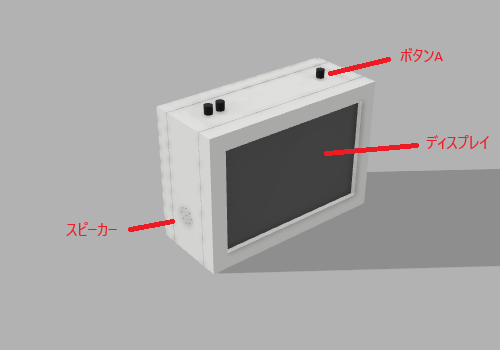
\includegraphics[width=100mm]{images/cad1.png}\\
  \caption{デバイス構想}
  \label{fig:cad1}
\end{figure}\\
\begin{figure}[htbp]
  \centering % 図を中央寄せにする
  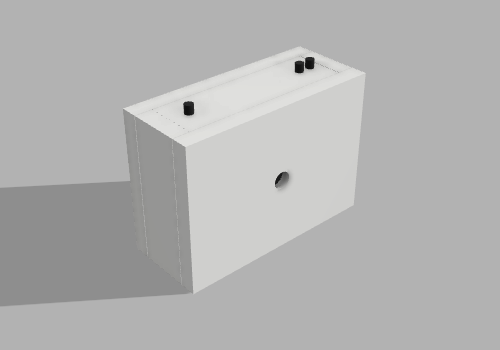
\includegraphics[width=100mm]{images/cad2.png}\\
  \caption{デバイス構想}
  \label{fig:cad2}
\end{figure}\\
昨今、デジタルデバイドにより、デジタル機器を扱うことが難しい方も少なくはない。
このデバイスは、デジカメの形を模した形となっており、高齢者等も直感的に使えるデバイスを目指している。
\Writer{金子康一}

\newpage

\subsection{システム構成}
\label{allSystem}
\noindent\space
また、次の\ref{convertArt}, \ref{convertMusic}節で説明する機能を実現するために、図\ref{fig:allSystem}の構成で、開発を行う。

\begin{figure}[htbp]
  \centering % 図を中央寄せにする
  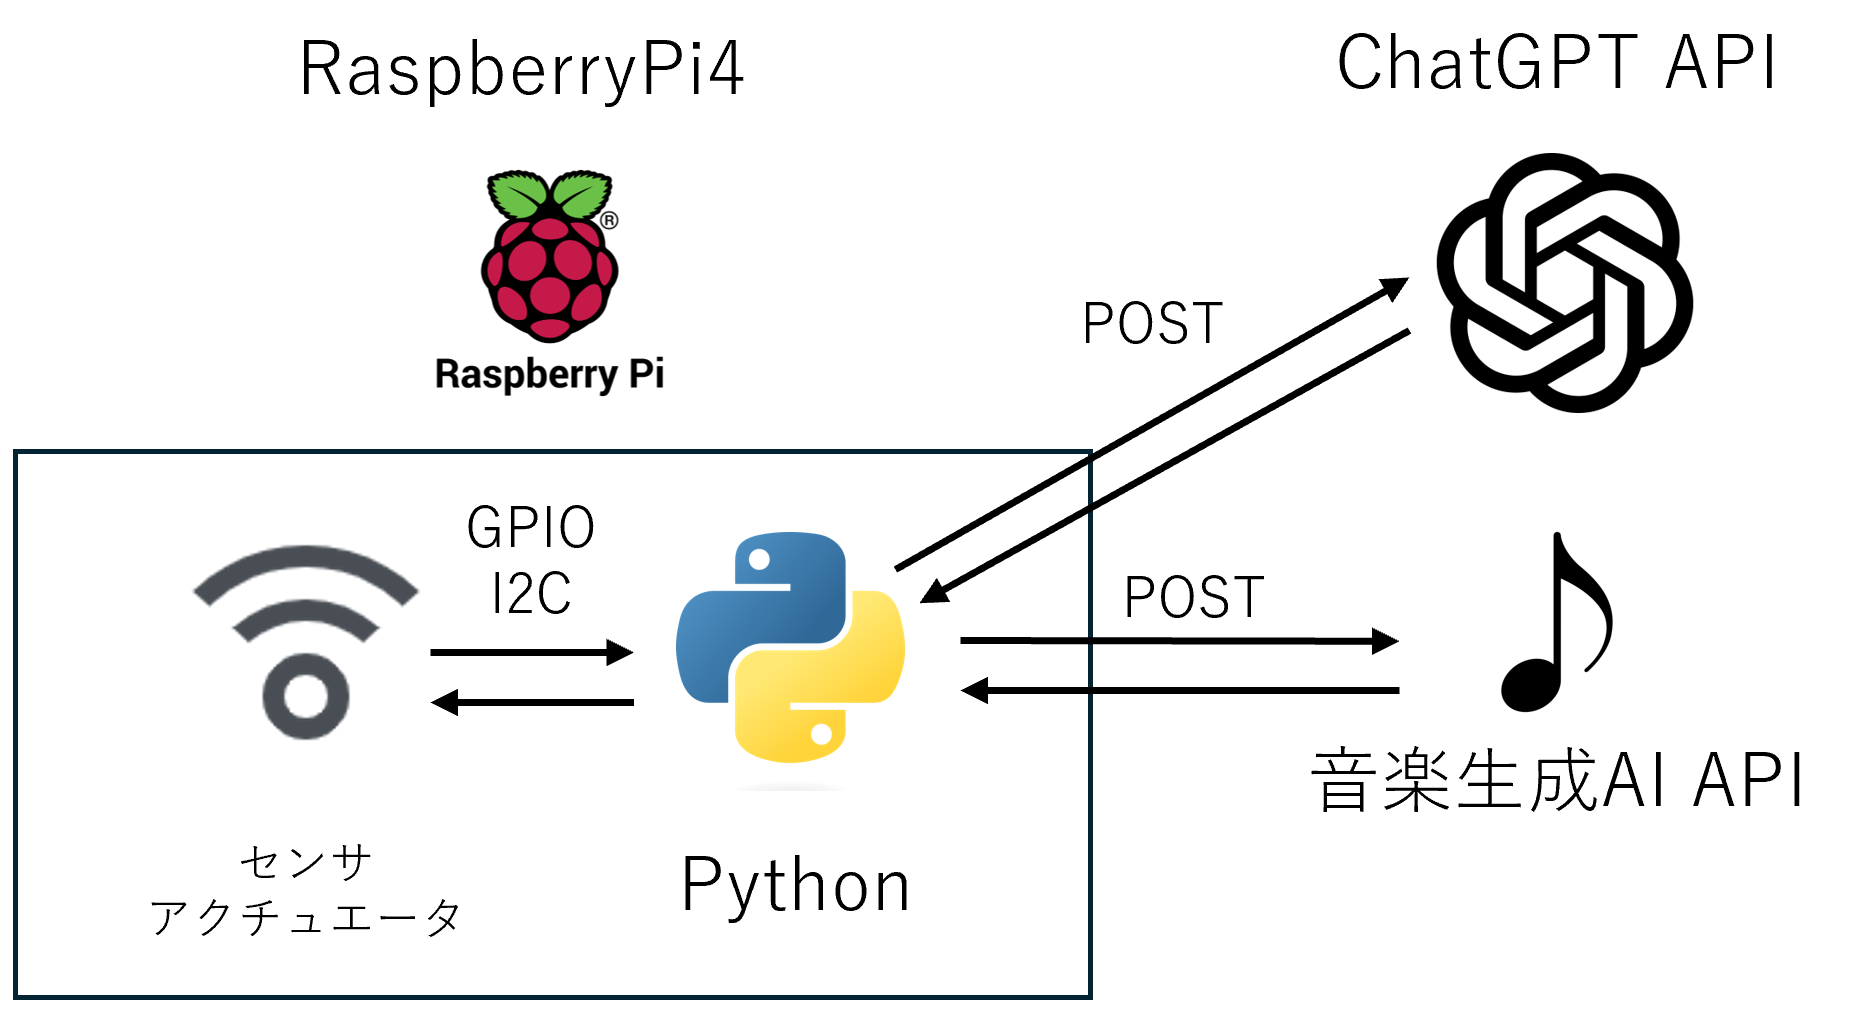
\includegraphics[width=100mm]{images/tech-conf.png}\\
  \caption{技術構成}
  \label{fig:allSystem}
\end{figure}
\noindent\space
デバイス本体を制御するために、シングルボードマイコンであるRaspberryPi 4を使用する。
また、RaspberryPi 4の制御はPython使用し、各センサ、アクチュエータとi2C通信もしくは、GPIOを通じて通信、制御を行う。

\Writer{金子康一}

\newpage

\subsection{聴覚情報を視覚情報に変換}
\label{convertArt}
\noindent\space
聴覚情報、すなわち風の音や川の音などをマイクで取り込み、画像生成AIもしくは何らかの方法で画像としてのアート(以下「アート」)を生成し、デバイスのディスプレに表示をする。\\
以上を実現するために、次のような手順で変換を行う。
\begin{enumerate}
  \item RaspberryPiに接続されたボタンAを押す。
  \item RaspberryPiに接続されたマイクから音を録音する。
  \item RaspberryPiに接続されたボタンAを押す。
  \item RaspberryPiに録音を終了する。
  \item OpenAI APIへ録音した音声データとプロンプトをPOSTし、音声データをテキストへ変換する。
  \item 変換されたテキストを画像生成AI、もしくは自作のAPIへPOSTしアートへ変換する。
  \item APIから返ってきた画像をデバイスのディスプレイに表示する。
\end{enumerate}
OpenAI APIの使用については公式ドキュメント\cite{OpenAIAPI}を参考に使用する。
アートへ変換するためのAPIの確定ができていないため、早急に確定させたい。
\Writer{金子康一}

\subsection{視覚情報を聴覚情報に変換}
\label{convertMusic}
\noindent\space
視覚情報、すなわち花の色や木々の揺れなどをカメラで撮影し、音楽生成AIもしくは何らかの方法で曲を生成し、デバイスに接続されたスピーカーで再生する。\\
以上を実現するために、次のような手順で変換を行う。
\begin{enumerate}
  \item RaspberryPiに接続されたボタンAを押す。
  \item RaspberryPiに接続されたカメラで撮影をする。
  \item OpenAI APIへ撮影した画像データとプロンプトをPOSTし、画像データをテキストへ変換する。
  \item 変換されたテキストを音楽生成AI、もしくは自作のAPIへPOSTし曲へ変換する。
  \item APIから返ってきた音声データをデバイスに接続されたスピーカーで再生する。
\end{enumerate} 
OpenAI APIの使用については公式ドキュメント\cite{OpenAIAPI}を参考に使用する。
生成された曲が風景とマッチしているかどうかの評価方法、それによるプロンプトの調整等については未確定の部分があるため詰めていきたい。
また、どのような音楽生成AIを使用するか確定できていないため、早急に確定したい。
\Writer{金子康一}

\chapter{活動の要約}
\section{成果}
\subsection{開発するデバイス}
\noindent\space
フィールドワーク、ブレインストーミングを行うことにより、ペルソナやどのようなデバイスを開発するのかを明確に考えることが出来た。
ブレインストーミングではFigJamを用いて以下の図\ref{fig:figjam}のように行った。
\begin{figure}[htbp]
  \centering % 図を中央寄せにする
  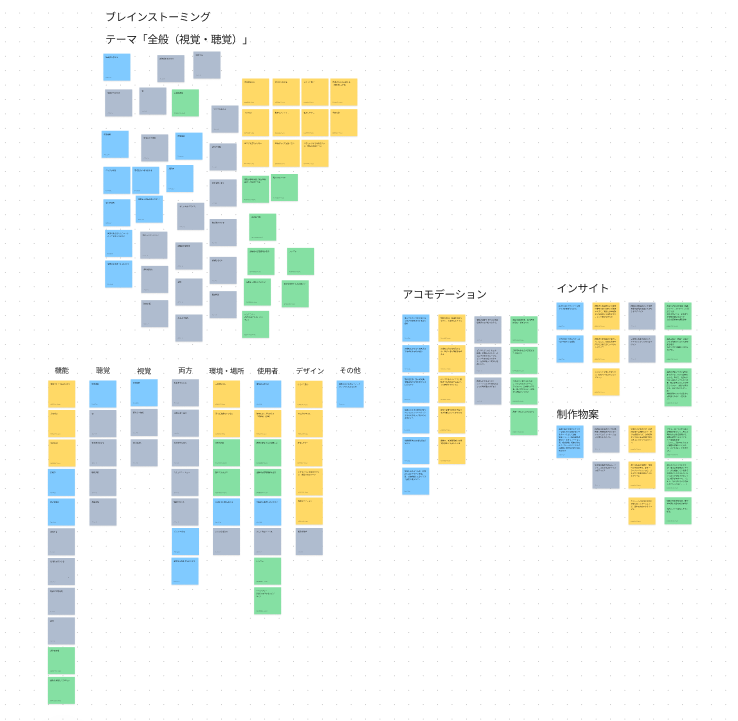
\includegraphics[width=100mm]{images/figjam.png}\\
  \caption{ブレインストーミング}
  \label{fig:figjam}
\end{figure}
\Writer{金子康一}

\subsection{システム設計}
\noindent\space
\ref{allSystem}節で述べた通り、システム構成を決めることが出来た。
生成系AIのAPIを活用することで、1年しかないプロジェクト学習の期間でも完成させることが出来ると考える。
\Writer{金子康一}

\subsection{ハードウェア設計}
\noindent\space
Fusion360を用いて完成イメージのCADを作成することが出来た。(図\ref{fig:cad1}, \ref{fig:cad2})
\Writer{金子康一}

\subsection{開発環境}
\noindent\space
開発をより円滑に効率的に行うために、以下の環境を用意した。
\begin{itemize}
  \item git
  \begin{itemize}
    \item コード等のバージョン管理に使用  
  \end{itemize}
  \item github
  \begin{itemize}
    \item 共同開発のために使用
    \item github Projectを活用したタスク管理や進捗の見える化を行いコミュニケーションコストを削減
  \end{itemize}
  \item Figma
  \begin{itemize}
    \item FigJamを使用したブレインストーミング等のアイデア出しで使用  
  \end{itemize}
  \item Cosence(旧ScrapBox)
  \begin{itemize}
    \item 活動等の記録に使用  
  \end{itemize}
  \item WSL Ubuntu
  \begin{itemize}
    \item LaTeXの環境
    \item ハードウェアを必要としないシステムの開発に使用  
  \end{itemize}
\end{itemize}
\Writer{金子康一}

\section{活動計画}\noindent
\subsection{全体(ワークショップ・イベント)}
\noindent\space
\begin{itemize}
  \item 5月
  \begin{itemize}
    \item プロジェクト配属
    \item グループ分け
  \end{itemize}
  \item 6月
  \begin{itemize}
    \item 視力障害支援者講習会
  \end{itemize}
  \item 7月
  \begin{itemize}
    \item 中間発表
    \item 中間報告
  \end{itemize}
  \item 後期
  \begin{itemize}
    \item 最終発表
    \item 最終報告
  \end{itemize}
\end{itemize}
\Writer{金子康一}

\subsection{ハードウェア}
\noindent\space
\begin{itemize}
  \item 5月
  \begin{itemize}
    \item RaspberryPi 4のセットアップ
    \item Visual Studio CodeからRemote SSHによる開発環境の構築
  \end{itemize}
  \item 6月
  \begin{itemize}
    \item 完成イメージCADの作成
    \item システム構成の構想
  \end{itemize}
  \item 7月
  \begin{itemize}
    \item RaspberryPi 4とカメラモジュール V3の接続確認
  \end{itemize}
  \item 後期
  \begin{itemize}
    \item 本体のCAD設計
    \item 回路設計・基盤発注
    \item 組み立て・制作
    \item 低レイヤー部分のプログラム開発
  \end{itemize}
\end{itemize}
\Writer{金子康一}

\subsection{ソフトウェア}
\noindent\space
\begin{itemize}
  \item 5月
  \begin{itemize}
    \item RaspberryPi 4のセットアップ
    \item Visual Studio CodeからRemote SSHによる開発環境の構築
  \end{itemize}
  \item 6月
  \begin{itemize}
    \item 音楽生成AI「Suno AI」の技術検証 
  \end{itemize}
  \item 7月
  \begin{itemize}
    \item 音楽生成AI「Stable Audio Open」のAPI使用を現時点で決定
  \end{itemize}
  \item 後期
  \begin{itemize}
    \item 画像生成AIの決定と技術検証
    \item OpenAIのAPI技術検証
    \item デバイスのソフトウェア部分のプログラミング開始
    \item RaspberryPi 4との連携
  \end{itemize}
\end{itemize}
\Writer{伊丸岡朝陽}

\newpage
\addcontentsline{toc}{chapter}{参考文献}
\begin{thebibliography}{1}
  \bibitem{先行研究} 峰野あゆみ(2013)「視覚障がい者の散策行動特性からみた支援環境に関する研究」,東京都立大学機関リポジトリ「みやこ鳥」(2024年7月10日取得, https://tokyo-metro-u.repo.nii.ac.jp/records/3633).
  \bibitem{OpenAIAPI} OpenAI. "Overview OpenAI API". OpenAI developer documentation. https://platform.openai.com/docs/overview. (2024/7/17アクセス).
\end{thebibliography}

\end{document}
